\chapter{ Strength in Numbers}
\label{les:15}

\begin{chapquote}{Lewis Carroll, \textit{Alice in Wonderland}}
``Let me see: four times five is twelve, and four times six is thirteen, and
four times seven is fourteen—oh dear! I shall never get to twenty at this
rate!''
\end{chapquote}

Numbers are an essential part of our everyday life. Large numbers,
however, aren't something most of us are too familiar with. The largest
numbers we might encounter in everyday life are in the range of
millions, billions, or trillions. We might read about millions of people
in poverty, billions of dollars spent on bank bailouts, and trillions of
national debt. Even though it's hard to make sense of these headlines,
we are somewhat comfortable with the size of those numbers.

Although we might seem comfortable with billions and trillions, our
intuition already starts to fail with numbers of this magnitude. Do you
have an intuition how long you would have to wait for a
million/billion/trillion seconds to pass? If you are anything like me,
you are lost without actually crunching the numbers.

Let's take a closer look at this example: the difference between each is an
increase by three orders of magnitude: $10^6$, $10^9$, $10^{12}$. Thinking about
seconds is not very useful, so let's translate this into something we can wrap
our head around:

-  $10^6$: One million seconds was $1 1/2$ weeks ago.
-  $10^9$: One billion seconds was almost 32 years ago.
-  $10^{12}$: One trillion seconds ago Manhattan was covered under a [thick
    layer of ice].

\begin{figure}
  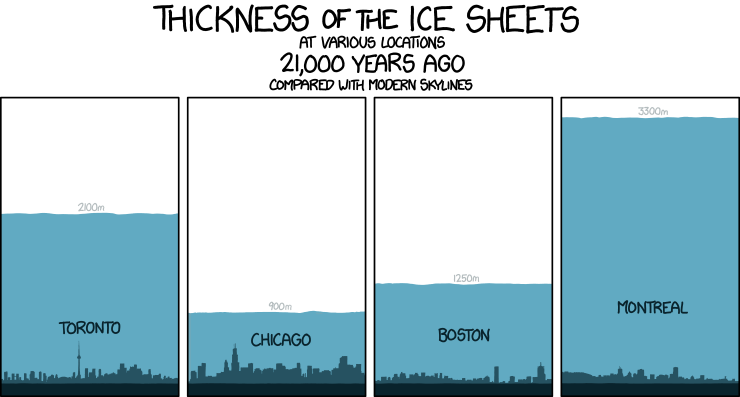
\includegraphics{assets/images/xkcd-1125.png}
  \caption{About 1 trillion seconds ago. Source: xkcd #1125}
  \label{fig:xkcd-1125}
\end{figure}

As soon as we enter the beyond-astronomical realm of modern
cryptography, our intuition fails catastrophically. Bitcoin is built
around large numbers and the virtual impossibility of guessing them.
These numbers are way, way larger than anything we might encounter in
day-to-day life. Many orders of magnitude larger. Understanding how
large these numbers truly are is essential to understanding Bitcoin as a
whole.

Let's take [SHA-256], one of the [hash functions] used in Bitcoin, as a
concrete example. It is only natural to think about 256 bits as "two
hundred fifty-six," which isn't a large number at all. However, the
number in SHA-256 is talking about orders of magnitude --- something our
brains are not well-equipped to deal with.

While bit length is a convenient metric, the true meaning of 256-bit
security is lost in translation. Similar to the millions ($10^6$) and
billions ($10^9$) above, the number in SHA-256 is about orders of magnitude
($2^{256}$).

So, how strong is SHA-256, exactly?

\begin{quotation}
``SHA-256 is very strong. It's not like the incremental step from MD5
to SHA1. It can last several decades unless there's some massive
breakthrough attack.''
\end{quotation}
% > <cite>[Satoshi Nakamoto]</cite>

Let's spell things out. $2^{256}$ equals the following number:

\begin{quotation}
    115 quattuorvigintillion 792 trevigintillion 89 duovigintillion 237
    unvigintillion 316 vigintillion 195 novemdecillion 423 octodecillion 570
    septendecillion 985 sexdecillion 8 quindecillion 687 quattuordecillion 907
    tredecillion 853 duodecillion 269 undecillion 984 decillion 665 nonillion
    640 octillion 564 septillion 39 sextillion 457 quintillion 584 quadrillion 7
    trillion 913 billion 129 million 639 thousand 936.
\end{quotation}

That's a lot of nonillions! Wrapping your head around this number is
pretty much impossible. There is nothing in the physical universe to
compare it to. It is far larger than the number of atoms in the
observable universe. The human brain simply isn't made to make sense of
it.

One of the best visualizations of the true strength of SHA-256 is the
following video by Grant Sanderson. Aptly named ["How secure is 256 bit
security?"] it beautifully shows how large a 256-bit space is. Do
yourself a favor and take the five minutes to watch it. As all other
[3Blue1Brown] videos it is not only fascinating but also exceptionally
well made. Warning: You might fall down a math rabbit hole.

% 

[Bruce Schneier] used the physical limits of computation to put this
number into perspective: even if we could build an optimal computer,
which would use any provided energy to [flip bits perfectly], build a
[Dyson sphere] around our sun, and let it run for 100 billion billion
years, we would still only have a 25% chance to find a needle in a
256-bit haystack.

\begin{quotation}
``These numbers have nothing to do with the technology of the devices;
they are the maximums that thermodynamics will allow. And they
strongly imply that brute-force attacks against 256-bit keys will be
infeasible until computers are built from something other than matter
and occupy something other than space.''
\end{quotation}
% > <cite>[Bruce Schneier][2]</cite>

It is hard to overstate the profoundness of this. Strong cryptography
inverts the power-balance of the physical world we are so used to.
Unbreakable things do not exist in the real world. Apply enough force,
and you will be able to open any door, box, or treasure chest.

Bitcoin's treasure chest is very different. It is secured by strong
cryptography, which does not give way to brute force. And as long as the
underlying mathematical assumptions hold, brute force is all we have.
Granted, there is also the option of a global [\$5 wrench attack][wrench attack].
But torture won't work for all bitcoin addresses, and the cryptographic
walls of bitcoin will defeat brute force attacks. Even if you come at it
with the force of a thousand suns. Literally.

This fact and its implications were poignantly summarized in the [call
to cryptographic arms][]: "*No amount of coercive force will ever solve
a math problem."*

\begin{quotation}
``It isn't obvious that the world had to work this way. But somehow the
universe smiles on encryption.''
\end{quotation}
% > <cite>[Julian Assange][call to cryptographic arms]</cite>

Nobody yet knows for sure if the universe's smile is genuine or not. It
is possible that our assumption of mathematical asymmetries is wrong and
we find that [P actually equals NP], or we find surprisingly quick
solutions to [specific problems] which we currently assume to be hard.
If that should be the case, cryptography as we know it will cease to
exist, and the implications would most likely change the world beyond
recognition.

\begin{quotation}
``Vires in Numeris'' = ``Strength in Numbers''
\end{quotation}
% > <cite>[epii]</cite>

*Vires in numeris* is not only a catchy motto used by bitcoiners. The
realization that there is an unfathomable strength to be found in
numbers is a profound one. Understanding this, and the inversion of
existing power balances which it enables changed my view of the world
and the future which lies ahead of us.

One direct result of this is the fact that you don't have to ask anyone
for permission to participate in Bitcoin. There is no page to sign up,
no company in charge, no government agency to send application forms to.
Simply generate a large number and you are pretty much good to go. The
central authority of account creation is mathematics. And God only knows
who is in charge of that.

% 

Bitcoin is built upon our best understanding of reality. While there are
still many open problems in physics, computer science, and mathematics,
we are pretty sure about some things. That there is an asymmetry between
finding solutions and validating the correctness of these solutions is
one such thing. That computation needs energy is another one. In other
words: finding a needle in a haystack is harder than checking if the
pointy thing in your hand is indeed a needle or not. And finding the
needle takes work.

The vastness of Bitcoin's address space is truly mind-boggling. The
number of private keys even more so. It is fascinating how much of our
modern world boils down to the improbability of finding a needle in an
unfathomably large haystack. I am now more aware of this fact than ever.

Bitcoin taught me that there is strength in numbers.

% ---
%
% #### Down the Rabbit Hole
%
% - [How secure is 256 bit security?]["How secure is 256 bit security?"] by 3Blue1Brown
% - [Block Hashing Algorithm][hash functions] on the Bitcoin Wiki
% - [Last Glacial Maximum][thick layer of ice], [SHA-2][SHA-256], [Dyson Sphere][Dyson sphere], [Landauer's Principle][flip bits perfectly] [P versus NP][P actually equals NP], [Discrete Logarithm][specific problems] on Wikipedia
%
% [thick layer of ice]: https://en.wikipedia.org/wiki/Last_Glacial_Maximum
% [xkcd \#1125]: https://xkcd.com/1225/
% [SHA-256]: https://en.wikipedia.org/wiki/SHA-2
% [hash functions]: https://en.bitcoin.it/wiki/Block_hashing_algorithm
% [Satoshi Nakamoto]: https://bitcointalk.org/index.php?topic=191.msg1585#msg1585
% ["How secure is 256 bit security?"]: https://www.youtube.com/watch?v=S9JGmA5_unY
% [Bruce Schneier]: https://www.schneier.com/
% [flip bits perfectly]: https://en.wikipedia.org/wiki/Landauer%27s_principle#Equation
% [Dyson sphere]: https://en.wikipedia.org/wiki/Dyson_sphere
% [2]: https://books.google.com/books?id=Ok0nDwAAQBAJ&pg=PT316&dq=%22These+numbers+have+nothing+to+do+with+the+technology+of+the+devices;%22&hl=en&sa=X&ved=0ahUKEwjXttWl8YLhAhUphOAKHZZOCcsQ6AEIKjAA#v=onepage&q&f=false
% [wrench attack]: https://xkcd.com/538/
% [call to cryptographic arms]: https://cryptome.org/2012/12/assange-crypto-arms.htm
% [P actually equals NP]: https://en.wikipedia.org/wiki/P_versus_NP_problem#P_=_NP
% [specific problems]: https://en.wikipedia.org/wiki/Discrete_logarithm#Cryptography
% [epii]: https://bitcointalk.org/index.php?topic=4994.msg140770#msg140770
% [3Blue1Brown]: https://twitter.com/3blue1brown
%
% <!-- Wikipedia -->
% [alice]: https://en.wikipedia.org/wiki/Alice%27s_Adventures_in_Wonderland
% [carroll]: https://en.wikipedia.org/wiki/Lewis_Carroll
